% Search for all the places that say "PUT SOMETHING HERE".

\documentclass[11pt]{article}
\usepackage{amsmath,textcomp,amssymb,geometry,graphicx,enumerate}

\def\Name{Aniket Ketkar, Tanay Lathia, Eric Priest, Steve Wang}  % Your name
\def\SID{24795502}  % Your student ID number
\def\Login{aniket.ketkar@berkeley.edu} % Your login (your class account, cs170-xy)
\def\Homework{3} % Number of Homework
\def\Session{Fall 2015}


\title{Statistics 133 - Final Project - "Team Feelin' the Bern"}
\author{\Name}
\markboth{Stat 133--\Session\  Final Project \Name}{ \Name}
\pagestyle{myheadings}
\date{}

\newenvironment{qparts}{\begin{enumerate}[{(}a{)}]}{\end{enumerate}}
\def\endproofmark{$\Box$}
\newenvironment{proof}{\par{\bf Proof}:}{\endproofmark\smallskip}

\textheight=9in
\textwidth=6.5in
\topmargin=-.75in
\oddsidemargin=0.25in
\evensidemargin=0.25in


\begin{document}
\maketitle

\section*{Abstract}


\section*{Background}

\section*{Questions for Analysis}

\section*{Methods}

\section*{Exploratory Analysis}

\section*{Machine Learning - K Nearest Neighbors - Equations}
K Nearest neighbors is a nonparametric machine learning technique to find similar points in a dataset. It makes the assumption that similar points will have similar results, so point's label is predicted as the average label of its neighbors. Check out \texttt{knn.R} for the team's implementation of KNN. \\ 
KNN does not make any assumptions about the structure of the dataset, underlying trends, or high level ideas. It just finds the nearest neighbors. For large datasets, like the one in this paper, KNN must run through all of the training points before it can make a prediction. Performance is guaranteed to be linear ($O(nf)$) with the size of the training data $n$ and number of features $f$. The more features, the farther points will be in space due to the curse of dimensionality, so we had to cut down on the featureset to make predictions better. \\ 

Let a single data point be $\mathbf{x_i} = (f_1, f_2, f_3...)$, in entire dataset $\mathbf{X}$. Then for training data point $\mathbf{x_j}$ for $i \neq j$, define the L2 distance metric for a single training example as $t_j = \sqrt{\Sigma(\mathbf{x_i} - \mathbf{x_j})^2}$. The training point $\mathbf{x_j}$ with minimum $t_j$ is the closest example to the desired prediction point. 

The algorithm is: 

\begin{enumerate}
\item For all $i \neq j$, compute $t_j$ 
\item Find $k$ smallest $t_j$ 
\item Return average of these $k$ values. 
\end{enumerate}

As you can see, this involves the entire training set. For state level predictions, we removed the state we are predicting on, leaving approximately 1600 counties to predict on. Each state prediction takes approximately 4 minutes (approximately 20 individual predictions). 

Despite the downsides, KNN performed much better than chance. Assuming two people races, a uniform assumption has expected win rate of 0.5, but every state had at least 70\% success, with some over 90%. 

\section*{Trump v Cruz Plots}
\textbf{Trump's data worked mostly well with KNN.} Below are some examples of states. The predictions are on the left, the actual results are on the right. Darker blue areas correspond to his predicted wins. \\

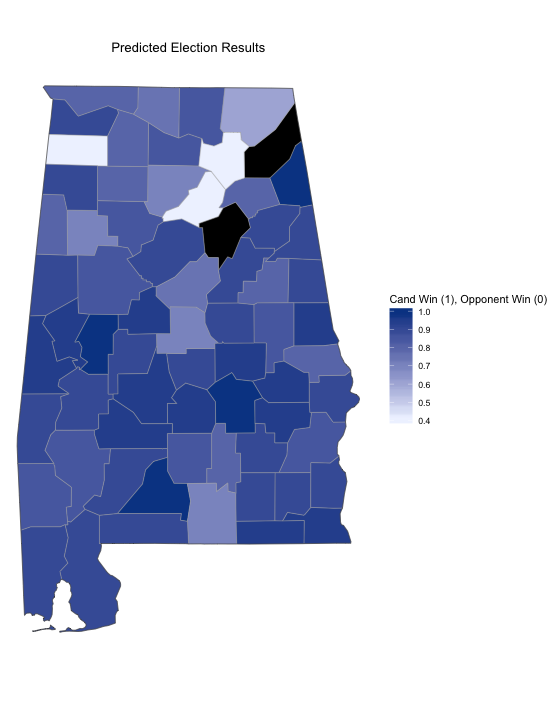
\includegraphics[scale=0.4]{../knn_plots/alabama_predicted.png} 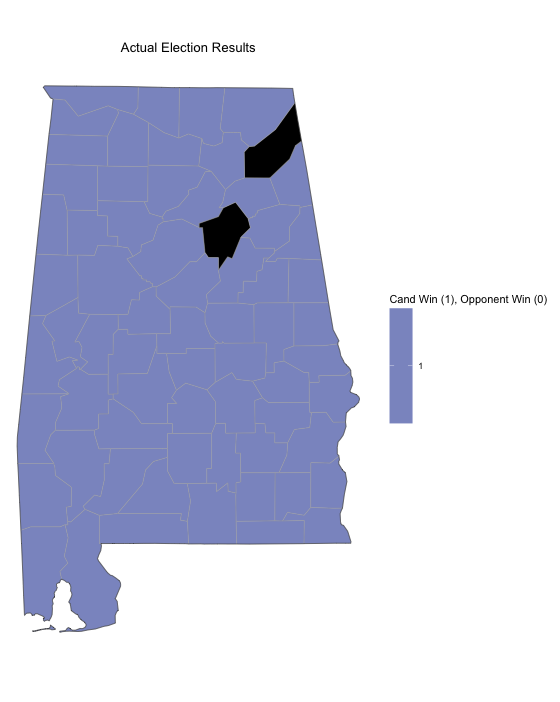
\includegraphics[scale=0.4]{../knn_plots/alabama_actual.png}\\
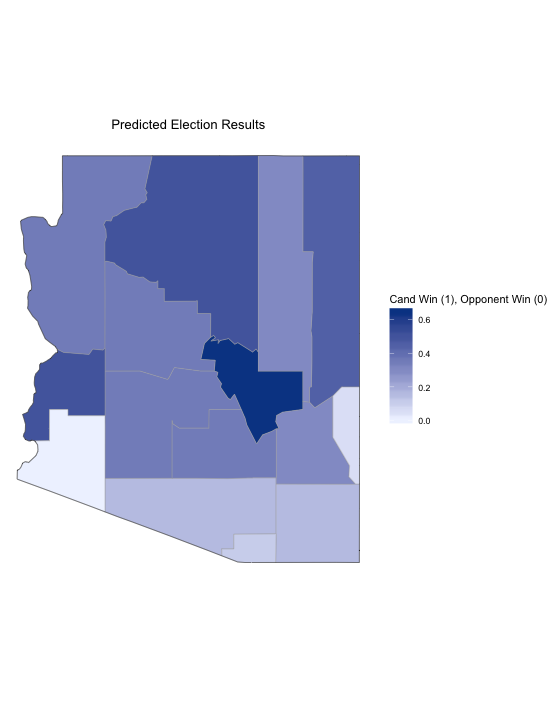
\includegraphics[scale=0.4]{../knn_plots/arizona_predicted.png} 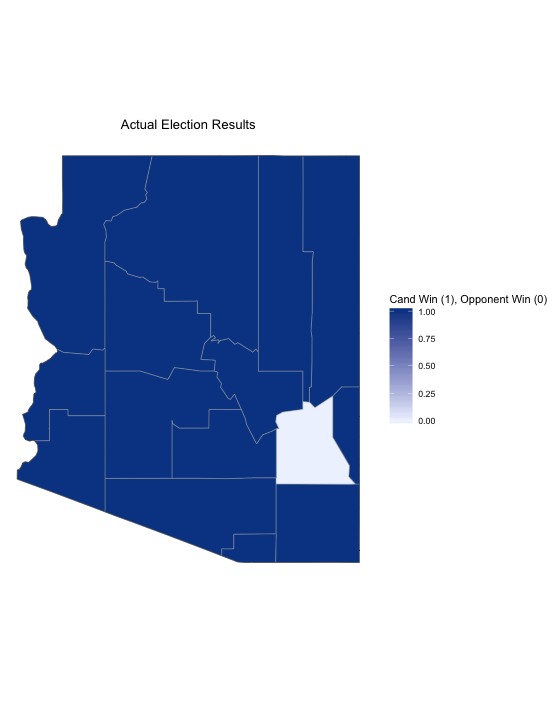
\includegraphics[scale=0.4]{../knn_plots/arizona_actual.png}\\
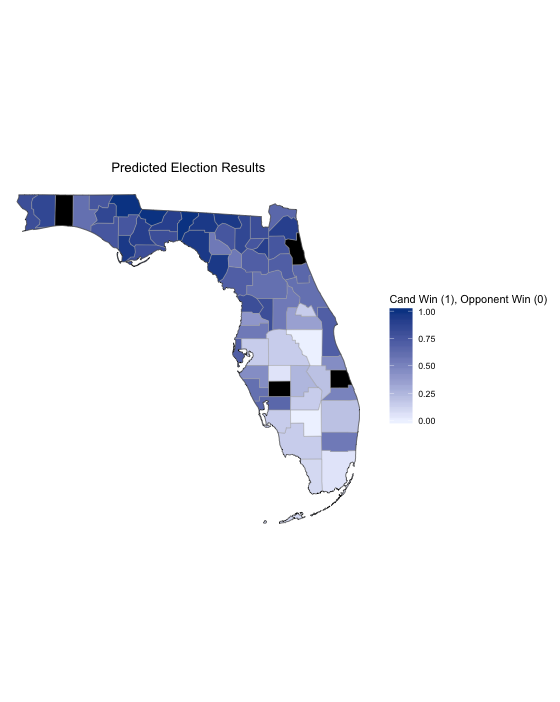
\includegraphics[scale=0.4]{../knn_plots/florida_predicted.png} 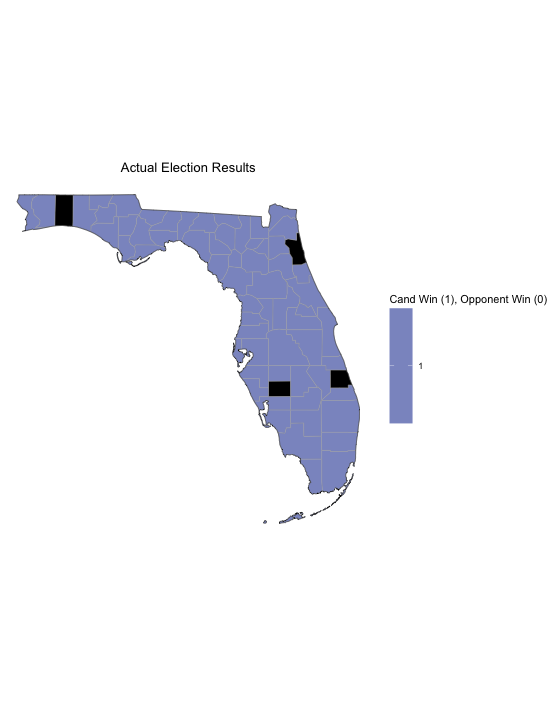
\includegraphics[scale=0.4]{../knn_plots/florida_actual.png}\\
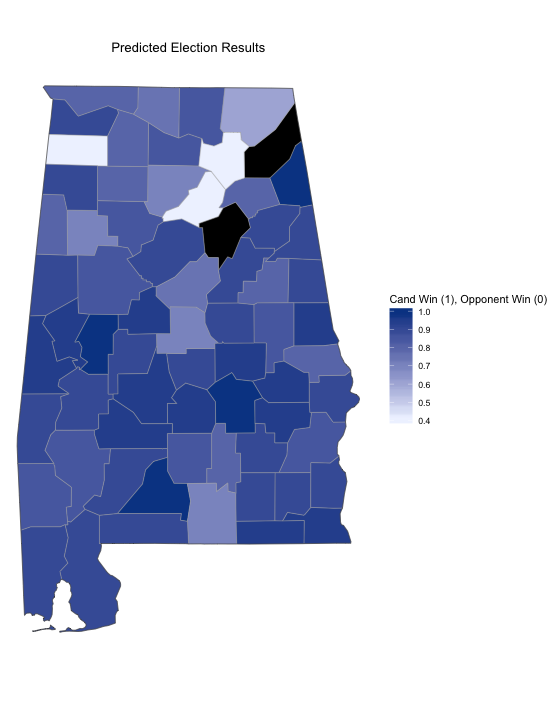
\includegraphics[scale=0.4]{../knn_plots/alabama_predicted.png} 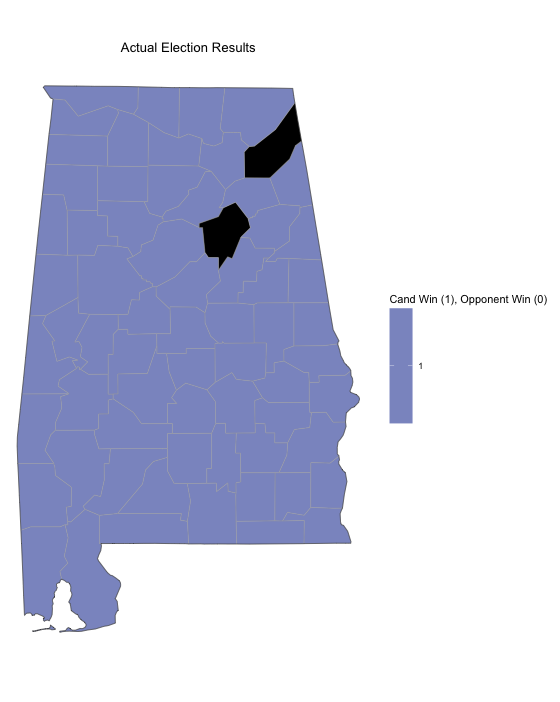
\includegraphics[scale=0.4]{../knn_plots/alabama_actual.png}\\
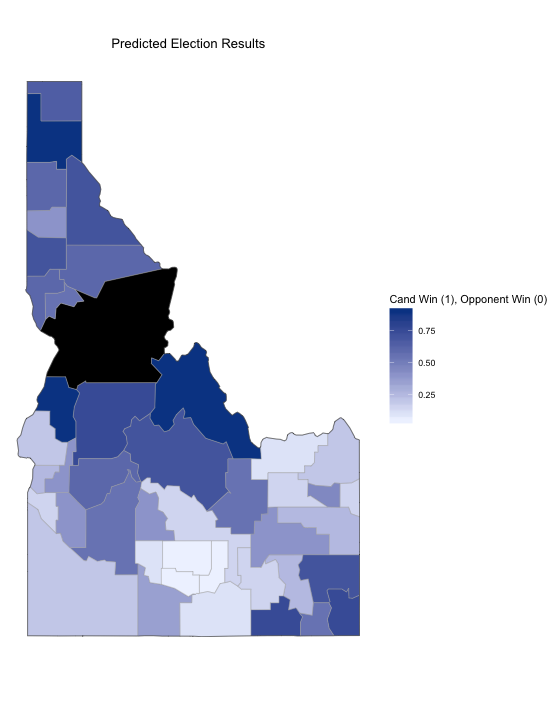
\includegraphics[scale=0.4]{../knn_plots/idaho_predicted.png} 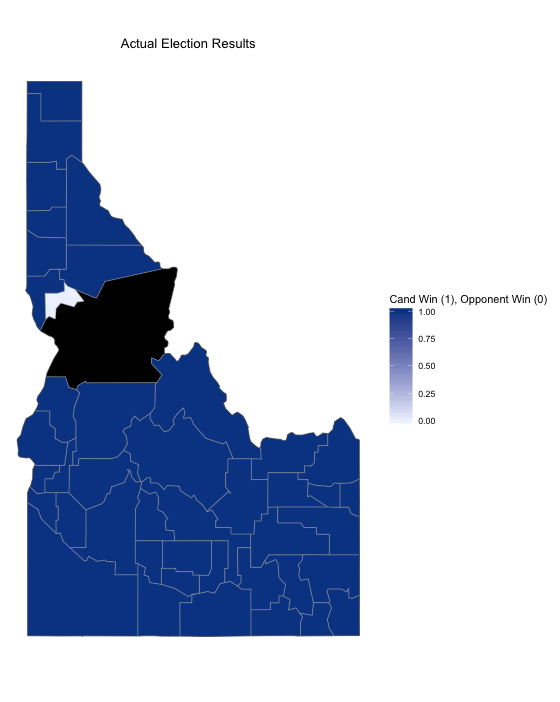
\includegraphics[scale=0.4]{../knn_plots/idaho_actual.png}\\


\section*{Sanders v Clinton Plots}
\textbf{The model somewhat works for Democratic candidates. } Here are the predictions for Sanders: \\
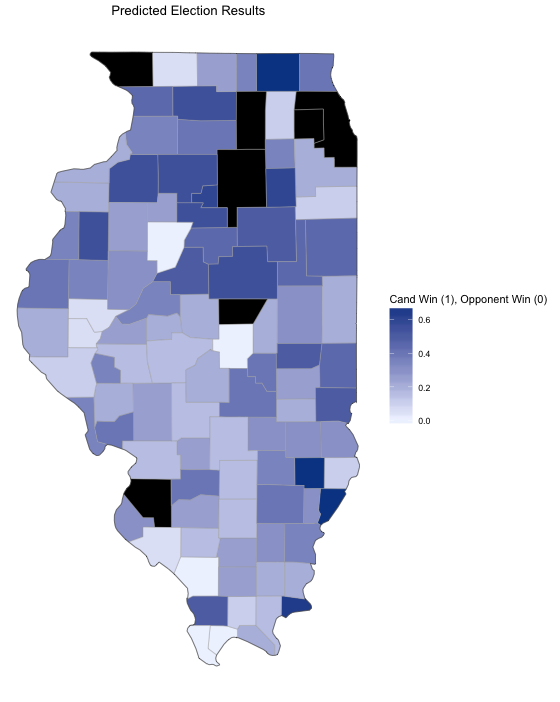
\includegraphics[scale=0.4]{../knn_plots/illinois_predicted.png} 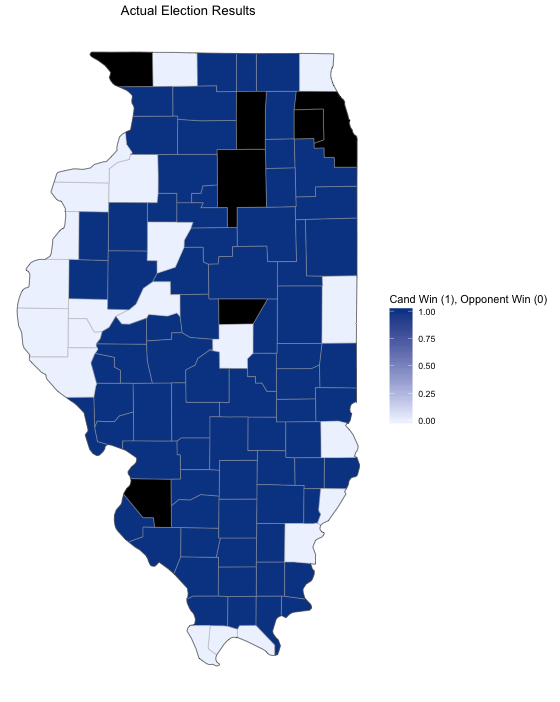
\includegraphics[scale=0.4]{../knn_plots/illinois_actual.png}\\
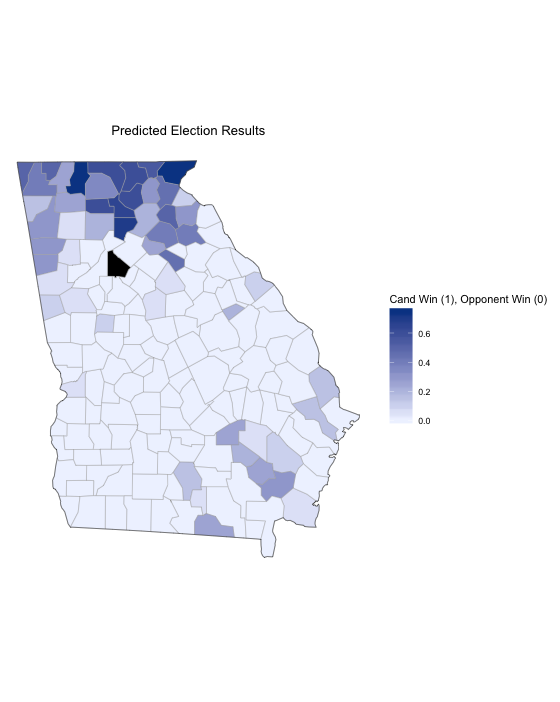
\includegraphics[scale=0.4]{../knn_plots/georgia_sanders_predicted.png} 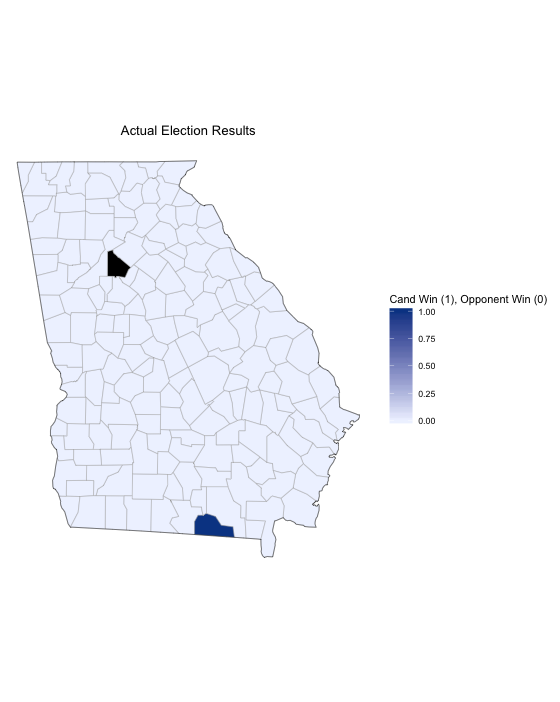
\includegraphics[scale=0.4]{../knn_plots/georgia_sanders_actual.png}\\

\section*{KNN Analysis}
The model works on a macro scale for each state, correctly predicting the majority of counties. It does well for homogeneous states, or states with clear demographic boundaries. A homogenous example is Sander's overwhelming loss in Georgia, since the counties are small and similar to each other and other Southern Clinton wins. Illinois has high variance between Chicago and other counties, and Northern states split more evenly between Sanders and Clinton, so the neighbors were split as well, leading to poorer performance. 

The model also worked somewhat well for Republican candidates, in particular in Idaho. Idaho's central regions voted for Trump and the periphery voted for Cruz, and the KNN model accurately captures this pattern. This is a big success for the model. 

Overall, the model works well when the training data is relatively homogenous. If a candidate has clearly won similar states, the model correctly predicts that they will win future similar states. In addition, if there are clear boundaries within a state, the model will pick up on that fact. 
\section*{Final Analysis - Answering the Questions}


\end{document}
